%!TEX root=../main.tex
% Chapter Template

\chapter{Implementation} % Main chapter title

\label{Chapter5} % Change X to a consecutive number; for referencing this chapter elsewhere, use \ref{ChapterX}

%----------------------------------------------------------------------------------------
%	SECTION 1
%----------------------------------------------------------------------------------------

\section{Solution overview}

The final solution consists of a \gls{REST} API build with ASP.NET Core and a MongoDB \gls{NoSQL} database. Both are hosted through Amazon Webservices in an EC2 container using Docker. \\
The API consists of the commands seen in appendix \ref{APICommands}. \\\\

This section covers the process from the initial data delivery to the final solution in a chronological order.

\section{Initial data dump}
In the beginning of the project we were supplied with data from one of \gls{Struct}' customers. This data was in the form of many SQL tables and most of the data was not relevant for creating product recommendations. The main tables used were the following:  \\
\begin{itemize}
\item Visitor: A collection of every unique visitor who had visited the customer's website, each visitor gets a unique identifier called UID. Contains 3,073,665  visitors.
\item Profile: A collection of every users signed up at the website. Contains 3037 profiles.
\item BehaviorData: A collection of every unique action performed by visitors on the website, for example when a visitor views a product a new row is made with the visitor's UID, the product UID and the timestamp. Contains 3,326,736 visitor actions.
\item Order: Contains each profile's orders. Contains 5520 orders.
\item Product: A collection of all products on the website with their unique IDs. Contains 22,445 products.
\item ProductGroup: A collection of all product groups. Contains 262 product groups.
\item AttributeValueRendered: A collection of product and product group descriptions in different languages. Contains 409,259 descriptions:

\end{itemize}

A snapshot of the visitor and behaviorData table can be seen in figure \ref{visitorTable} and \ref{behaviorTable}.

\begin{figure}[H]
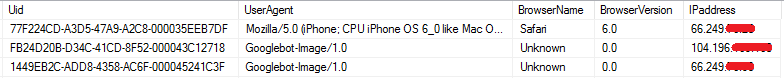
\includegraphics[scale=0.8]{Visitor_table}
\caption{Visitor table from the original data}
\label{visitorTable}
\end{figure}
\begin{figure}[H]
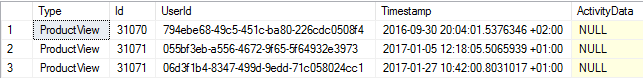
\includegraphics{behaviorData_table}
\caption{Behavior data table from the original data}
\label{behaviorTable}
\end{figure}

These tables contain all the pertinent information for creating product recommendations and can be utilized after a cleaning and structuring process. This process is described in the following sections.

\section{Data Transformation}
To begin the initial data transformation a data storing technology has to be selected. The technology chosen was \gls{NoSQL}, specifically \gls{MongoDB} the most popular No-SQL framework \cite{DBRankings}. \\
\gls{NoSQL} is chosen because of the good fit for this project. The data demands are not clearly specified in the beginning and with No-SQL it is easy to add or remove data or even change the data types on the fly. No-SQL's denormalized format also allows for faster retrieval of a single item without having to do joins or complex SQL queries. Finally No-SQL is easier to scale across multiple servers and many engines have built in scaling functionalities \cite{SQLvsNOSQL} which can come in handy when multiple clients begin using the service. \\\\

A brief overview of the different terminology for SQL and No-SQL is given in table \ref{sqlvsnosql_table}.
\begin{table}[H]
\centering
\caption{SQL vs No-SQL terminology}
\label{sqlvsnosql_table}
\begin{tabular}{|l|l|p{8cm}|}
\hline
\textbf{SQL}   & \textbf{No-SQL}     & \textbf{Comment}                                                                                                    \\ \hline
Table & Collection &                                                                                                            \\ \hline
Row   & Document   & A No-SQL document can contain more complex datatype compared to a row in SQL e.g arrays or other documents \\
\hline
\end{tabular}
\end{table}

Python was used to accomplish the early migration from SQL tables to MongoDB. Several scripts were created to retrieve the data from the SQL server and transfer it to the MongoDB database in the wanted format. Pseudo code of one of these scripts can be seen in appendix \ref{PythonScript}. \\

After all the scripts are finished the No-SQL database has the collections Visitor and Product. A breakdown of documents in the two collections can be seen in table \ref{documents}	

\begin{table}[H]
\centering
\caption{An overview of the fields in each document in the collections}
\label{documents}
\begin{tabular}{|l|l|p{7cm}|}
\hline
\textbf{Document} & \textbf{Fields}                                                                                                                          & \textbf{Comment}                                                                   \\ \hline
Visitor           & \begin{tabular}[c]{@{}l@{}}Id: string\\ Behaviors: array\\ ProfileUID: string\\ CustomerUID: string\end{tabular}                         & The behavior array is an array of Behavior documents which contains all the behaviors of the specific visitor \\ \hline
Product           & \begin{tabular}[c]{@{}l@{}}Id: int\\ ProductGroupId: int\\ VisitorId: stringArray\\ Description: string\\ Created: DateTime\end{tabular} &     The visitorId array contains Ids of all visitors who have looked at this product    \\ \hline
Behavior & \begin{tabular}[c]{@{}l@{}}Type: string \\ Id: int \\ Timestamp: DateTime \end{tabular} & A behavior document holds information about a particular behavior \\ \hline
\end{tabular}
\end{table}

An example of a Visitort document can be seen in figure \ref{visitorDoc} and an example of a Product document can be seen in appendix \ref{productDoc}.
\begin{figure}[H]
\centering
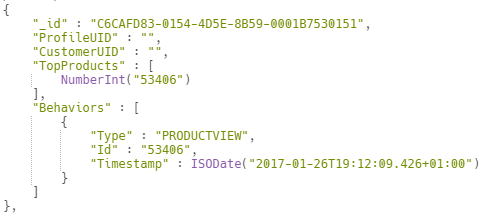
\includegraphics{visitorDocument}
\caption{A Visitor document example}
\label{visitorDoc}
\end{figure}

The topProducts array seen in appendix \ref{productDoc} was not part of the original data transformation, but rather a part of the recommendation algorithm explanied later in this chapter.

After the data has been cleaned and structured in No-SQL the algorithm for determining product recommendations can be made. The algorithm is described in the following section.

\section{The product recommendation algorithm}
There are multiple ways to implement af product recommendation algorithm all with their advantages and disadvantages. The method chosen for this project is called Item-to-Item collaborative filtering. Other methods and the reasoning why these weren't chosen is described in further detail in Chapter 6 discussion. \\\\

Item-to-Item collaborative filtering is a datamining tool to link items (products) with other items in terms of their similarity. This method is also the way \gls{Amazon} handles their product recommendations \cite{AmazonRecommendations}. \\
The specifics of the algorithm differs from implementation to implementation. In this version each product is compared to other products based on how much they have been viewed together by customers, the likeness of their description and their product group. \\
The first run of the algorithm requires going through each product and the visitors of each product to see what else they have looked at. This needs a lot of resources, but once run only new behavior has to be re-calculated. A run down of the algorithm can be seen in algorithm \ref{alg:collaborativeFilter}. \\\\

\begin{algorithm}[H]
\caption{Item-to-Item collaborative filtering algorithm}
\label{alg:collaborativeFilter}
\begin{algorithmic}[!H]
\ForAll{Products p}
\State productScores = Dictionary<int, double>
\ForAll{Visitors in p}
\ForAll{Products visitorProduct in Visitor behaviors}
\If{productScores contains visitorProduct}
\State productScores[visitorProduct]++
\Else
\State productScores.Add(visitorProduct, 1)
\EndIf
\EndFor
\EndFor
\State Sort productScores after highest value
\ForAll{Products similarProduct in productScores}
\State productScores[similarProduct] = \textbf{calculateSimilarityScore(p, similarProduct, productScores[similarProduct])} (see algorithm \ref{alg:calculateSimilarity})
\EndFor
\State Sort productScores after highest value
\State Store top 10 productScores in database under p
\EndFor
\end{algorithmic}
\end{algorithm}

\begin{algorithm}[H]
\caption{Similarity calculations for two products }
\label{alg:calculateSimilarity}
\begin{algorithmic}[!H]

\State \textbf{calculateSimilarityScore(mainProduct p1, compareProduct p2, currentScore)}
\State similarAttributeFactor = 0.02
\State productGroupFactor = 0
\State numOfSimAttributes = 0
\If{p1.productGroup equals p2.productGroup}
\State productGroupFactor = 0.02
\EndIf
\ForAll{words w in p1.description}
\If{w is in p2.description}
\State numOfSimAttributes++
\EndIf
\EndFor
\If{numOfSimAttributes equals 0}
\State similarAttributeFactor = 0
\EndIf
\State \textbf{return} \begin{math} currentScore * (1+productGroupFactor)*(1+similarAttributeFactor^{numOfSimAttributes}) \end{math}
\end{algorithmic}
\end{algorithm}


After algorithms \ref{alg:collaborativeFilter} and \ref{alg:calculateSimilarity} each product in the database now has an array with the top 10 similar products based on amount of views, description and product group. \\
Next up is calculating the top products for each visitor, these are the products the specific visitor has viewed the most. This is accomplished by iterating through each visitor, checking their behavior and storing their top products as a field in the database. This calculation can be seen in algorithm \ref{alg:topProducts}. This calculation also requires a large amount of resources the first time, but very little to maintain.

\begin{algorithm}[H]
\caption{Calculations of each visitors top products}
\label{alg:topProducts}
\begin{algorithmic}[H]
\ForAll{Visitors v}
\State visitorProducts = Dictionary<string, int>
\ForAll{Behaviors b in v}
\State topVistorProducts[b.Id]++
\EndFor
\State Sort visitorProducts after highest value
\State Store top 5 visitorProducts in database under v
\EndFor
\end{algorithmic}
\end{algorithm}

Since all these calculations are made before the actual product recommendations are requested, the process of recommending products is quite fast. The recommendation process starts with retrieving the requested visitor's top products from the database, retrieving these products top similar products, sorting them based on their score and finally returning the amount asked for. The code for the recommendation part can be seen in algorithm \ref{alg:recommendation}

\begin{algorithm}[H]
\caption{Get product recommendations}
\label{alg:recommendation}
\begin{algorithmic}[H]
\State visitorTopProducts = db.GetTopProducts(visitorUID)
\State productRecommendations = Dictionary<int, double>
\ForAll{Products p in visitorTopProducts}
\State SimilarProducts = db.GetTopProductRecommendation(product)
\ForAll{products simProduct in similarProducts}
\If{productRecommendations contains simProduct}
\State productRecommendations[simProduct] += similarProducts[simProduct]
\Else
\State productRecommendations.add(simProduct, similarProducts[simProduct]
\EndIf
\EndFor
\EndFor
\State Sort productRecommendations after highest value
\State \textbf{return} amount of productRecommendations requested
\State 
\end{algorithmic}
\end{algorithm}

The entire process of requesting product recommendation, running algorithm \ref{alg:recommendation} and returning them takes less than 40ms which satisfies the non-functional requirement NF02. \\\\
Some other paths are required in certain situations such as when the visitor does not have any behavior or not enough behavior to satisfy the amount of recommendations requested. In these cases the remaining recommendations are filled from the top 20 most popular products in the last 30 days. The top 20 products are calculated by checking the timestamp and finding those in the last 30 days and then counting how many times each product was viewed. The top 20 products are stored in the database and can be calculated through an API call.

\section{Handling new data}
When new visitors are created or new behavior is discovered the client has to call the corresponding API functions in order to store this data alongside the other. When new behavior data is registered the program re-calculates the visitor in question's top product as well as the product in question's similar products. This way the algorithm is always up to date and the calculations can happen asynchronously and thereby have no affect the load times for the end user.

\section{Hosting the API}
An API can be hosted in several different ways, through many providers. This product recommendation API is hosted through Amazon WebServices in an \gls{EC2Instance} \cite{EC2}. To accomplish this the ASP.NET core project is built in a Docker container, the container is pushed to the Docker Hub and then pulled and run in the \gls{EC2Instance}. The database is similarly packed in a docker container and run in the \gls{EC2Instance}. The Docker containers have exposed ports to the rest of the internet and can be accessed via \gls{EC2Instance} public DNS or IP.



			


 